\documentclass[12pt,fleqn]{article}
\input{/home/clair/Documents/definitions}

%----------------------------------------------------------------------
% SPECIFY BIBLIOGRAPHY FILE & FIELDS TO EXCLUDE
\addbibresource{vonMises.bib}
\AtEveryBibitem{\clearfield{url}}
\AtEveryBibitem{\clearfield{doi}}
\AtEveryBibitem{\clearfield{isbn}}
\AtEveryBibitem{\clearfield{issn}}

%----------------------------------------------------------------------
% REFORMAT HEADERS
\titleformat{\section}
	{\normalfont\bfseries}
%	{\llap{\parbox{1cm}			% offsets section number in margin
	{\thesection}{1em}{}
	
\titleformat{\subsection}
	{\normalfont\bfseries}
	{\llap{\parbox{1cm}{\thesubsection}}}{0em}{}

%=====================================================================

\begin{document}
\section{Circular distributions}

Any data set in which the observations can be represented as points on a circle is a circular data set. The observations may be measured angles, or may be cyclical observations of another kind, such as the time of year at which events of interest occur. Simply treating such data as existing on a finite linear support is not appropriate, since our choice of where on the circle our linear support begins and ends will affect the results obtained; instead, specific circular distributions must be used.

The circular analogue to the normal distribution is the wrapped normal distribution, in which a linear normal distribution with support $(-\infty, \infty)$ is wrapped onto a unit circle. However, the circular distribution thus obtained is rather complicated, and unlike the standard normal distribution, does not belong to the exponential family; a more natural choice, far more commonly used for circular data, is the von Mises distribution, which can be used to closely approximate the wrapped normal distribution (and other distributions, such as cardioid distributions) and does belong to the exponential family, so is much more tractable mathematically. 

%--------------------------------------------------------------------------------

\section{The von Mises distribution}
A von Mises distribution of an angle $\theta$ is usually written $\theta \sim M(\mu, \kappa)$, its two parameters being the circular mean $\mu$ and the concentration $\kappa$, and has probability density function
\[g(\theta ; \mu, \kappa) = \frac{e^{\kappa \cos(\theta - \mu)}}{2\pi I_0(\kappa)}\]
with $I_0(\kappa)$ the modified Bessel function of the first kind and order $p=0$, where:
\[I_p(\kappa) = \frac{1}{2\pi} \int_0^{2\pi} \cos(p\theta) e^{\kappa \cos \theta} d\theta \]

Although negative values of $\kappa$ are theoretically admissible, the convention is to take $\kappa > 0$, since $M(\mu, \kappa)$ and $M(\mu+\pi, -\kappa)$ give the same distribution of $\theta$. This also lends itself to a simple, intuitive interpretation of the concentration parameter; when $\kappa = 0$, the distribution of $\theta$ is uniform about the circle, growing more concentrated about $\mu$ as $\kappa$ increases. When $\kappa = 1$, 78\% of the distribution will lie within $\pi/2$ radians of the mode at $\mu$, increasing to more than 99\% for $\kappa = 4$. The ratio of the density of the mode at $\mu$ to that of the antimode at $\mu \pm \pi$ is $e^{2\kappa}$.

Figure~\ref{fig:vM-density-plots} shows von Mises distributions with the same circular mean and a range of concentration parameters, both in their circular form (\ref{fig:vM-circular-density}) and on a linear axis\footnote{When creating a linear plot of circular data the cutpoint used is essentially arbitrary, but since we are generally interested in the mode of the data, it makes sense to cut at the antimode, at $\mu \pm \pi$ - or $\bar{\theta} \pm \pi$, for sampled data.} (\ref{fig:vM-linear-density}), where the degree of concentration for each $\kappa$ is much easier to discern by eye. 


\begin{figure}[h!]
\caption{Densities of von Mises distributions with $\mu = 0$ and varying values of $\kappa$.}
\label{fig:vM-density-plots}
\begin{subfigure}[t]{0.5\textwidth}
\caption{Circular density}
\label{fig:vM-circular-density}
\centering
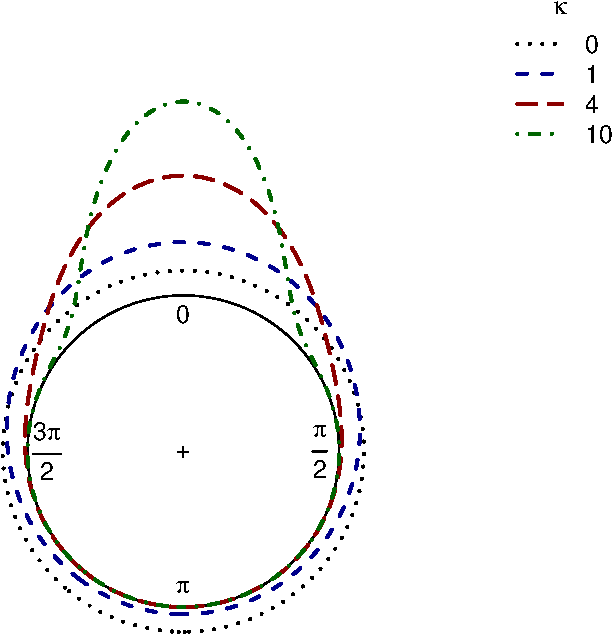
\includegraphics[scale = 0.5, keepaspectratio]{vM-circular-plot-crop.pdf}
\end{subfigure}
\begin{subfigure}[t]{0.5\textwidth}
\caption{Converted to linear form}
\label{fig:vM-linear-density}
\centering
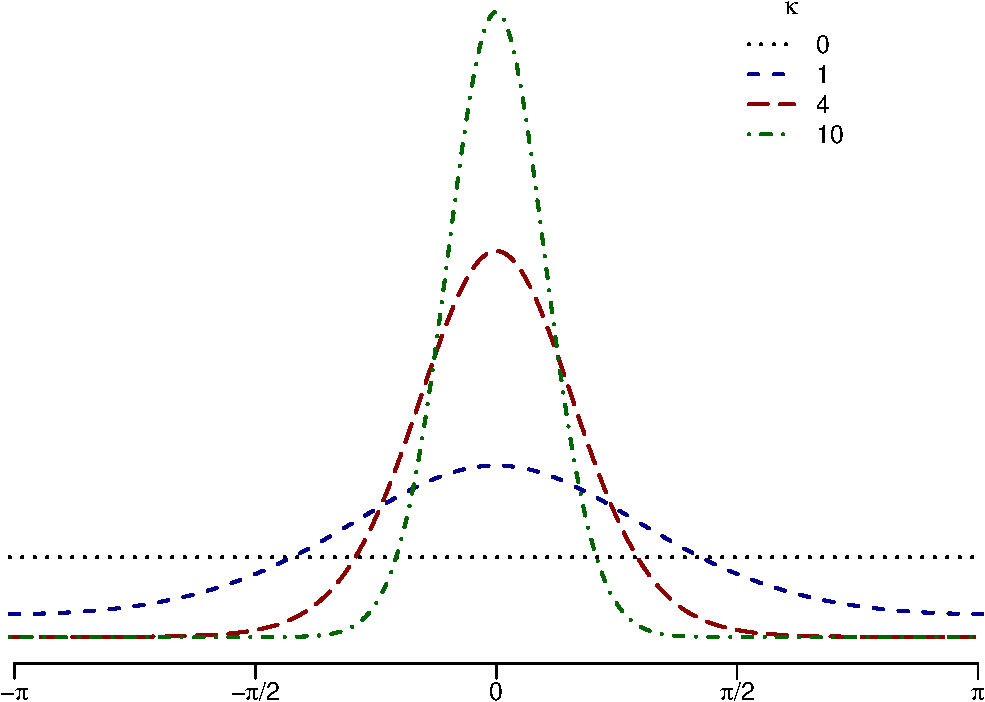
\includegraphics[width=0.9\textwidth, keepaspectratio]{vM-linear-plot-crop.pdf}
\end{subfigure}
\end{figure}



%--------------------------------------------------------------------------------

\section{Summary statistics}

For circular distributions, estimating the sample mean is not as simple as in the linear case; we can't simply sum the observations and divide by $n$, since the resulting value would depend on the reference point against which the angles were measured.

To obtain a sample mean that is invariant under rotation, we instead consider each $\theta_j$ as the angle of a unit vector $\mathbf{x}_j$; this representation is known as the embedding approach (as opposed to the intrinsic approach, which represents the directions by angles). We can easily find the mean resultant vector $\mathbf{\bar{x}}$, which has its centre of mass at Cartesian coordinates $(\bar{C}, \bar{S})$, where

\vspace{-10pt}
\begin{minipage}{0.5\linewidth}
\[\bar{C} = \frac{1}{n} \sum_{j=1}^{n} \cos \theta_j,\]
\end{minipage}
\hspace{0.5cm}
\begin{minipage}{0.5\linewidth}
\[\bar{S} = \frac{1}{n} \sum_{j=1}^{n} \sin \theta_j.\]
\end{minipage}

We can use these to find the mean resultant length $\bar{R} = (\bar{C}^2 + \bar{S}^2)^{1/2}$; then $\bar{\theta}$ is the solution of $\bar{C} = \bar{R} \cos \bar{\theta}$ and $\bar{S} = \bar{R} \sin \bar{\theta}$. 
When $\bar{R} = 0$, $\bar{\theta}$ is undefined, so for $\bar{R} > 0$ we have 
\[ \bar{\theta} = \left\{ \begin{matrix*}[l]
\tan^{-1}(\bar{S}/\bar{C}) & \text{if }\bar{C} \geq 0 \\
\tan^{-1}(\bar{S}/\bar{C}) + \pi & \text{if }\bar{C} < 0 
\end{matrix*} \right. \]

%\nb{Sufficiency?}


Since all of the vectors $\mathbf{x}_j$ are unit vectors, it must be the case that $0 \leq \bar{R} \leq 1$; so we can use this statistic as an approximate measure of the concentration of the angles observed; if the values are clustered together tightly, then $\bar{R}$ will be close to 1, while if they are widely dispersed, $\bar{R}$ will be close to 0. However, if we observe $\bar{R} = 0$, we cannot assume that the directions are spread evenly around the circle; a sample containing clusters of opposing angles $\theta_1, \dots, \theta_n$ and $\theta_1+\pi, \dots, \theta_n+\pi$ will have $\bar{R} = 0$, but the angles are not uniformly distributed about the circle (a formal test of uniformity, as defined in \cite{Mardia1999}, would be required to confirm whether this is the case). %\nb{AXIAL DATA HANDLED HOW? BOTH TWO-WAY \& 4-WAY AXIAL?}

%--------------------------------------------------------------------------------

\section{Estimating parameters from observed data}

Given a sample of angles $\boldsymbol{\theta} = \theta_1, \dots, \theta_n$,  the parameters of the generating von Mises distribution are usually estimated using maximum likelihood methods. As we might intuitively expect, the maximum likelihood estimator of $\mu$ is $\hat{\mu} = \bar{\theta}$, and is unbiased. The MLE $\hat{\kappa}$ for the concentration parameter can be obtained using $\rho$, the population analogue of $\bar{R}$. Since $\rho = A(\kappa)$, $\bar{R} = A(\hat{\kappa})$, where $A(\hat{\kappa}) = I_1(\hat{\kappa})/I_0(\hat{\kappa})$ and $I_p(\hat{\kappa})$ is a modified Bessel function of order $p$, as defined previously. Thus we obtain the MLE $\hat{\kappa} = A^{-1}(\bar{R})$, which, although a biased estimator, is asymptotically unbiased. 


Since there is no closed-form expression for $A^{-1}(\cdot)$, various approximations to $\hat{\kappa}$ have historically been proposed (examples can be found in \cite{Mardia1999}); a function to carry out the necessary computation can be found in R's \texttt{circular} package, along with a range of other plotting and model fitting/generating tools (see \cite{Pewsey2014} for examples).

% \nb{Don't bother with marginal likelihood estimator $\check{\kappa}$ - not really useful at this point.}


%--------------------------------------------------------------------------------

\section{Bayesian inference on von Mises distributions}
Direct Bayesian inference on a von Mises distribution requires numerical methods because of the difficulty of evaluating the normalising constant. A joint conjugate von Mises prior for $\mu$ and $\kappa$ of
\[f(\mu, \kappa|\mathbf{\theta}) \propto \frac{1}{I_0(\kappa)^c} e^{\kappa R_0 \cos(\mu - \mu_0)} \]
where $c$ represents how many observations' worth of weight is placed on the prior, and  $\mu_0$ and $R_0$ are our prior estimates of $\mu$ and $\rho$, gives a von Mises posterior distribution for $\mu$, which can be sampled from using a number of established methods (for example, \cite{Best1979}), but the normalising constant for the posterior distribution of $\kappa$ is intractable, except in a limited number of cases.

Several Monte Carlo algorithms have been proposed, but most require a known concentration parameter and need some dataset-specific tuning. Damien and Walker \cite{Damien1999} propose a Gibbs sampler on an augmented state space that requires the addition of four latent variables before the full conditional posterior distributions can be obtained (but which has the advantages that it does not require tuning based on the data, and that all sampling is from uniform distributions), while \cite{Forbes2015} recently proposed a new algorithm for fast and efficient sampling from the posterior distribution of $\kappa$ by approximating the Bessel exponential distribution using a rejection sampler.

%\nb{couple of concluding lines?}

Bayesian inference is also frequently used to investigate mixtures of von Mises distributions, a method that can be applied to test the sensitivity of an assumed distribution to contamination with observations from another von Mises distribution, as in \cite{Bagchi1990}.

\newpage

\printbibliography

\end{document}
